\chaptercover{Experiment and Results}{chap:Results}
{In this chapter, we present several studies conducted during our investigation. In Section~\ref{Results-1} we explore the difficulty of learning OCL when compared to other subjects of SWEBOK, followed by an assessment of the variables that influence students' performance in OCL questionnaires, presented in Section~\ref{Results-2}. Section~\ref{chap:Results-OCLHighlightPlugin} concludes this chapter with the results of the influence of the OCL Highlight Plugin in these same questionnaires.}

\begin{comment}
Experiment 1: Relative Difficulty of Learning OCL
Experiment 2: Assessing OCL Comprehension
    - assessing the success and the duration
    Section 1: Metrics
    Section 2: plugin, model, grades
Experiment 3: On the Effect of Using the OCL Highlight Plugin
 Section 1: avaliação qualitativa dos professores
 Section 2: avaliaçao quantitativa das notas dos alunos
\end{comment}

%explore the concepts and the state of the art concerning the topics that relate to our intended work, which allow us to have a better understanding of the problem under study. This chapter is organized in 5 sections, structured as follows. Section~\ref{RelatedWork-1} starts by presenting the main concepts of Model-Driven Development, including the definition of UML, and OCL. Section~\ref{RelatedWork-2} covers some existing studies on UML class diagrams comprehension, including the impact of OCL on UML-based development. Section~\ref{RelatedWork-3} discusses the complexity of OCL expressions, and how it influences the cognitive effort. Section~\ref{RelatedWork-5} examines, in a broader perspective, relevant papers on the impact of syntax highlighting on program comprehension. Finally, Section~\ref{RelatedWork-5} presents the main OCL support tools and their most important functionalities.


%TODO: some introduction about the context

%We controlled for the origin of students since they were following two different degrees (computer science and business informatics) and the school year since although the overall degree and course syllabus have remained constant during the observation period, variations in students background might have occurred.



%\subsection{Evidence on the Relative Difficulty of Learning OCL}
\section{Experiment 1: Relative Difficulty of Learning OCL}
\label{Results-1}

In this section, we investigate the complexity of learning OCL when compared to a set of other Software Engineering topics offered in two university courses that together span a full school year. The courses' syllabuses were organized according to the following areas of SWEBOK: Software Requirements, Software Design, Software Construction, Software Testing, Software Maintenance, Software Configuration Management, Software Engineering Management, Software Engineering Process, Software Engineering Tools and Methods, Software Quality. Although OCL was taught as part of the Software Design area, it was considered separately in this study. In the Software Design area were kept other topics, namely the one of "Design Patterns".

After taking each area, learning was assessed through comprehensive questionnaires of closed true-false questions, through an e-learning system. Data was collected in two consecutive years, totalling around 150 students enrolled in four computer science-related graduations\footnote{The dataset used in this section is made available at \url{https://doi.org/10.5281/zenodo.4166133}}. Table~\ref{tbl:SWEBOKDescriptiveStatistics} presents descriptive statistics for the grades obtained in OCL and in the topics framed by the SWEBOK knowledge areas. The variability in the number of students per area is due to the fact that the tests for each topic took place throughout the semester, with some dropouts over time. Also, Software Requirements was taken only by students of 1 of the four graduations, and Software Construction was taken only by students of 3 of the four graduations, resulting in a smaller number of cases compared to the other topics.

% Please add the following required packages to your document preamble:
% \usepackage{booktabs}
\begin{table}[h]
\centering
\caption{Descriptive Statistics for the Learning Grades}
 \label{tbl:SWEBOKDescriptiveStatistics}
\resizebox{\textwidth}{!}{
\begin{tabular}{@{}lccccc@{}}
\toprule
\multicolumn{1}{c}{SWEBOK Area}   & N   & Minimum & Maximum  & Mean      & Std. Deviation \\ \midrule
OCL                               & 156 & 0,00\%  & 100,00\% & 50,9179\% & 33,50341\%     \\
Software Engineering Management   & 124 & 0,00\%  & 93,33\%  & 54,2314\% & 22,06163\%     \\
Software Quality                  & 159 & 0,00\%  & 94,44\%  & 54,3902\% & 21,03014\%     \\
Software Requirements             & 59  & 5,00\%  & 100,00\% & 58,1185\% & 21,84444\%     \\
Software Testing                  & 141 & 0,00\%  & 100,00\% & 60,4914\% & 22,06326\%     \\
Software Configuration Management & 133 & 0,00\%  & 100,00\% & 61,8988\% & 19,04061\%     \\
Software Engineering Process      & 132 & 0,00\%  & 95,00\%  & 65,1486\% & 14,14917\%     \\
Software Design                   & 121 & 0,00\%  & 100,00\% & 65,7350\% & 22,70123\%     \\
Software Construction             & 103 & 14,29\% & 100,00\% & 67,7011\% & 21,92754\%     \\ \bottomrule
\end{tabular}
}
\end{table}

\begin{comment}
    \begin{figure}[ht]
    \centering
    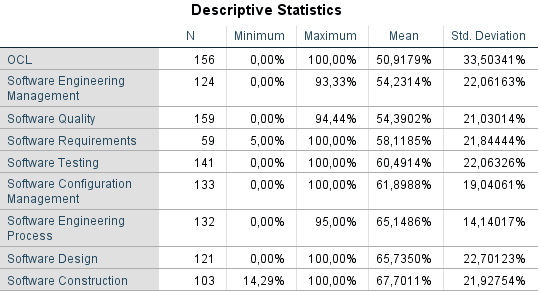
\includegraphics[width=0.8\textwidth]{figures/6_Results/Section1/01_GradesDescriptiveStatistics}
    \caption{Descriptive Statistics for the questionnaire grades}
    \label{fig:GradesDescriptiveStatistics}
    \end{figure}
\end{comment}

OCL was the topic were students obtained the worst grade, on average. To validate if the distribution of grades in OCL is significantly different from the ones obtained in the other topics, we started by performing a One-Sample Kolmogorov-Smirnov Test, with Lilliefors significance correction, to check if the grades obtained in the topics were normally distributed. The results did not allow to assume a normal distribution for most topics. Thus, a non-parametric Related-Samples Wilcoxon Signed Rank Test between the grades obtained in OCL and the remaining areas considered separately was applied. Results are shown in Table~\ref{tbl:OCLvsSWEBOK} for a significance level of 0.05, resulting in the decision of retaining the null hypothesis for Software Requirements, Software Engineering Management, and Software Quality.

\begin{table}[ht]
    \centering
    \begin{threeparttable}  
        \caption{Related-Samples Wilcoxon Signed Rank Test results (questionnaire grades in OCL versus in other SWEBOK topics)}
        
        \label{tbl:OCLvsSWEBOK}
        
        \begin{tabular}{@{}lcl@{}}
            \toprule
            
            SWEBOK Area & Test Sign. & Decision\\
            
            \midrule
            
            Software Requirements & .719 & Retain null hypot.\\
            
            Software Design & .000 & Reject null hypot.\\

            Software Construction & .000 & Reject null hypot.\\

            Software Testing & .011 & Reject null hypot.\\

            Software Maintenance & .026 & Reject null hypot.\\

%            \begin{tabular}[c]{m{3cm}}
                Software Configuration Management
%            \end{tabular}
            & .000 & Reject null hypot.\\

%            \begin{tabular}[c]{m{3cm}}
                Software Engineering Management
%            \end{tabular}
            & .187 & Retain null hypot.\\

            Software Engineering Process & .000 & Reject null hypot.\\

%            \begin{tabular}[c]{m{3cm}}
                Software Engineering Tools and Methods
%            \end{tabular}
            & .006 & Reject null hypot.\\
            
            Software Quality & .487 & Retain null hypot.\\

            \bottomrule
        
        \end{tabular}
        
    \end{threeparttable} 
\end{table}


A Friedman ANOVA test confirmed that there is no significant difference in the distribution of the grades obtained in OCL and in the SWEBOK topics of Software Requirements, Software Engineering Management and Software Quality, $\chi^2\mathrm{p}(3) = 4.86, \rho < 0.05$ (see Figure~\ref{fig:FriedmandANOVA}). 

\begin{figure}[ht]
\centering
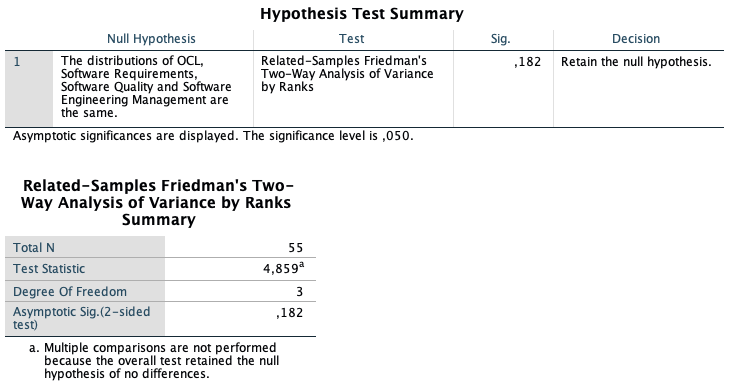
\includegraphics[width=1\textwidth]{Chapters/figures/6_Results/Section1/01_FriedmanANOVA.png}
\caption{Related Samples Friedman ANOVA Test}
\label{fig:FriedmandANOVA}
\end{figure}

From this analysis, we conclude that, despite the claims on OCL being challenging to learn, there are other topics in SWEBOK that reveal similar difficulty. However, as stated in the objectives section, this investigation will is focused on trying to soften the learning curve of OCL.

%\subsection{Analysis of collected data}
\section{Experiment 2: Assessing OCL Comprehension}
\label{Results-2}

\begin{comment}
Experiment 2: Assessing OCL Comprehension
    - assessing the success and the duration
    Section 1: Metrics
    Section 2: plugin, model, grades
\end{comment}   

The analysis presented in this section is based on the dataset\footnote{The collected dataset used in this section is made available at \url{http://xxx}} containing the data collected during five different school years (identified in Figure~\ref{fig:01_barchart_answersperschoolyear} with numbers from 1 to 5). During this five years, students of three different undergraduate university courses were given OCL questionnaires (with a limited duration of 40 minutes) built as follows, to guarantee a true-false answer: the same UML class model with no more than 20 classes (to fit legibly in a computer screen) was made available to all students of a course in advance, and its semantics explained in detail throughout the semester. In the day of the questionnaire, a large set of objects and links were given to students right before they start answering it. Students then instantiate the class model in USE and can make free use of it while answering the questionnaire. Each of its 10 NL questions (extracted randomly from a set of questions, to avoid cheating) could be answered by formulating a quantitative OCL expression upon the instantiated model. For instance, in an instantiated model of Royal and Loyal, the correct answer to \textit{"how many services are provided by TAP?"} would be 42, requiring the students to develop an OCL expression similar to Expression~\ref{lst:ocl_expression_3}. To be considered a correct answer, students had to fill that value in the e-learning platform. In each year, a different UML model was given: FootballCup on years 1 and 3, AirNova on years 2 and 5, and IULTrain on year 4. Models were created with similar complexity (comparable number of classes, including utility classes, and enumerations) to allow a fair assessment across the different school years. It's important to note that on school year 5 the OCL Highlight plugin was introduced to the students, not only for learning during the classes but also as a tool to assist them during the assignments.

\begin{lstlisting}[caption={OCL expression 3}\label{lst:ocl_expression_3}]

TAP.programs.levels.availableServices->size
\end{lstlisting}

\begin{figure}[ht]
\centering
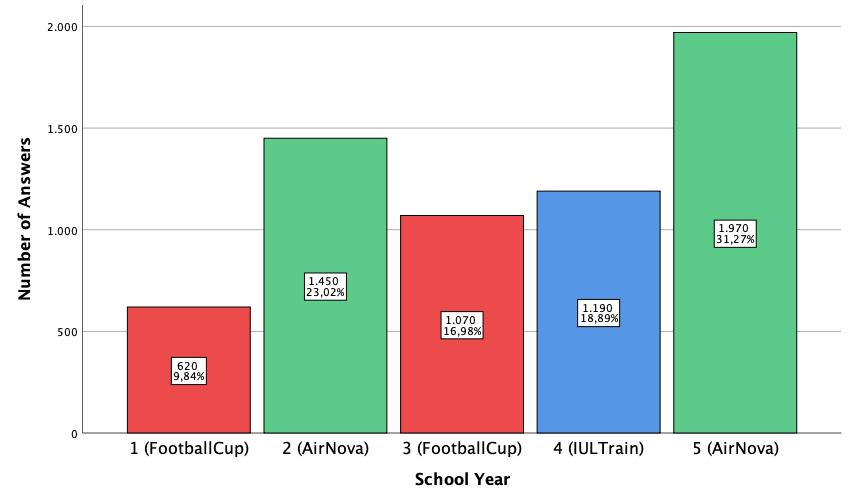
\includegraphics[width=1\textwidth]{Chapters/figures/6_Results/Section2/01_Barchart_AnswersPerYear.jpg}
\caption{Barchart of answers per school year}
\label{fig:01_barchart_answersperschoolyear}
\end{figure}

Figure~\ref{fig:02_barchart_answersperschoolyear} shows a Crosstabs of the percentage of correct answers across the different years. Years 3 and 5 have the highest percentage of correct answers, with 50.1\% and 54.5\% correct answers, respectively. Year 2, despite using the same model as in year 5, showed the smallest value of correct answers, with just 36.3\%. Years 1 and 3 studied the same model (FootballCup), but results don't show a significant difference (only 4\% more correct answers on Year 3, whereas from year 2 to 5 the difference is 18.2\%). 

\begin{figure}[ht]
\centering
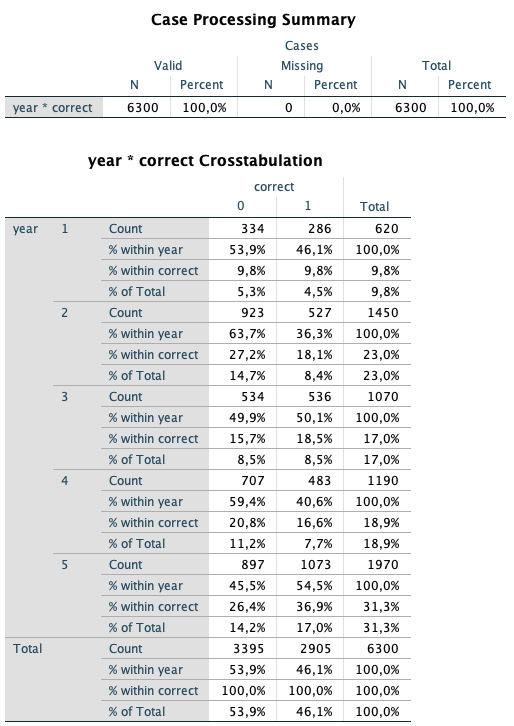
\includegraphics[width=0.7\textwidth]{Chapters/figures/6_Results/Section2/02_CrossTabs_CorrectnessPerYear.png}
\caption{Crosstabs of answers' correctness per school year}
\label{fig:02_barchart_answersperschoolyear}
\end{figure}

In the following subsections we present the studies conducted to analyze the influence of different metrics on the results of student's assessments across the years.

\subsection{OCL complexity metrics}
\label{Results-OCLComplexityMetrics}

As a first attempt, we analyse the influence of OCL complexity metrics on the success rate of student's assessments. From the dataset described above, we extracted the unique OCL expressions, in a total of 140, calculating for each of them its complexities using the OCL Complexity Plugin. Since many metrics were proposed in the literature (Section~\ref{sec:RelatedWork-Metrics}), we executed a variable reduction, not to obtain an overspecified model. 

Using a Kolmogorov-Smirnov test (see Figure~\ref{fig:02_ks_oclmetrics}) we examined the normality of the given metrics. For NNR, the results indicated that OCL metrics do not follow a normal distribution, D(140) = .19, p = .00 (other metrics showed similar results).

\begin{figure}[ht]
\centering
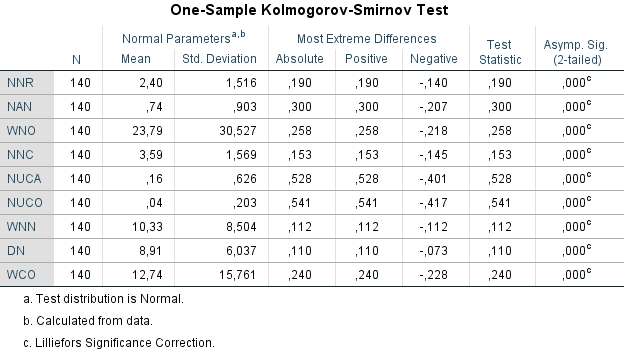
\includegraphics[width=1\textwidth]{Chapters/figures/6_Results/Section2/01_KS_OCLmetrics}
\caption{Kolmogorov–Smirnov test on the normal distribution of OCL complexity metrics}
\label{fig:02_ks_oclmetrics}
\end{figure}

To evaluate if these metrics can explain the success of students answers, and because the independent variables (metrics) don't follow a normal distribution, we applied a Spearman's rho correlation coefficient to evaluate their correlation, and their effect on the dependent variable (student's success). Figure~\ref{fig:01_sr_oclmetrics} presents the result of this test. Our decision was to exclude metrics with strong correlation, as they can be used to explain the same results, keeping the metrics that are more dissimilar (indentified in dark blue). The resulting metrics were NAN, WNO, NUCO, and WCO, as they reveal greater influence on the dependent variable.

\begin{figure}[ht]
\centering
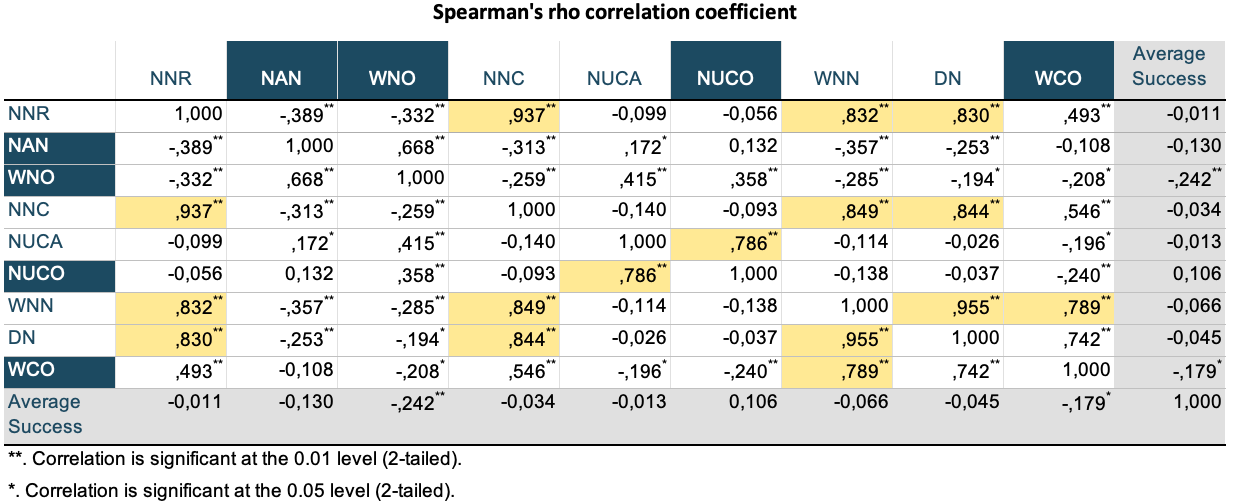
\includegraphics[width=1\textwidth]{Chapters/figures/6_Results/Section2/01_SR_OCLmetrics}
\caption{Spearman's rho correlation coefficient of OCL complexity metrics}
\label{fig:01_sr_oclmetrics}
\end{figure}

After reducing from nine to only four metrics, we performed a Linear Regression to assess the capability of the reduced set to explain the success of the students, as Spearman's rho can evaluate relative monotonies whether the models are linear or not. The results of this test are shown in Figure~\ref{fig:01_lr_oclmetrics}. A significant regression equation was found F(4, 135) = 4.313, $p<.01$, $R^{2}$ = .113, $R^{2}adjusted$ = .087. The resulting linear model revealed a poor explanatory power on the dependent variable (student's success), meaning that there is a monotony relationship, but it is not linear. The regression coefficient $B$ = .041 indicated that an increase in one point in NAN corresponded, on average, to an increase in student's success of .041 points (analogous analysis to other metrics).

\begin{figure}[ht]
\centering
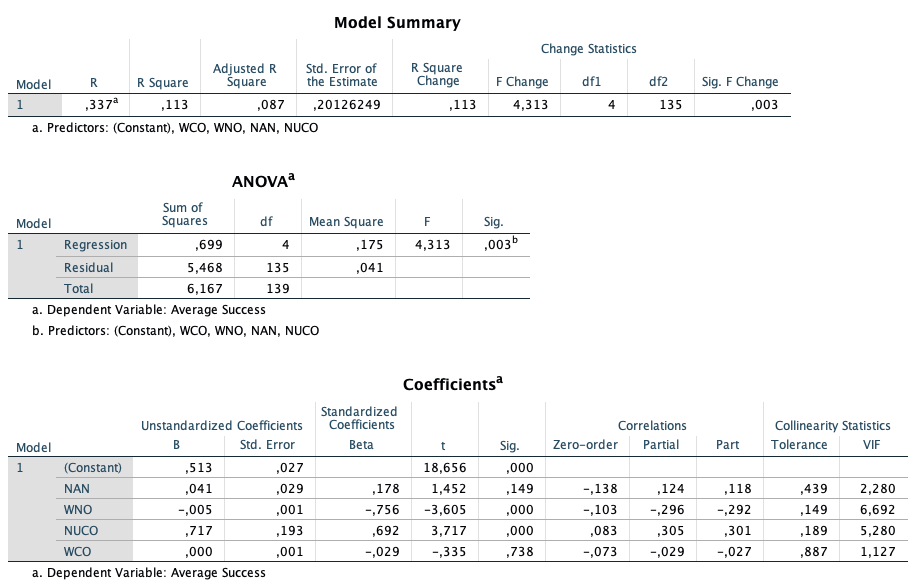
\includegraphics[width=1\textwidth]{Chapters/figures/6_Results/Section2/01_LR_OCLmetrics.png}
\caption{Linear Regression using NAN, WNO, NUCO, and WCO to explain the success}
\label{fig:01_lr_oclmetrics}
\end{figure}

Given the weak results of the first variable reduction, we opted for a Principal Component Analysis on the initial metrics that resulted in three components with a cumulative explanatory power of 90.986\% (Figure~\ref{fig:02_fa_oclmetrics}). The weight of each metric on the components can be seen in Figure~\ref{fig:02_cm_oclmetrics}. 

\begin{figure}[ht]
\centering
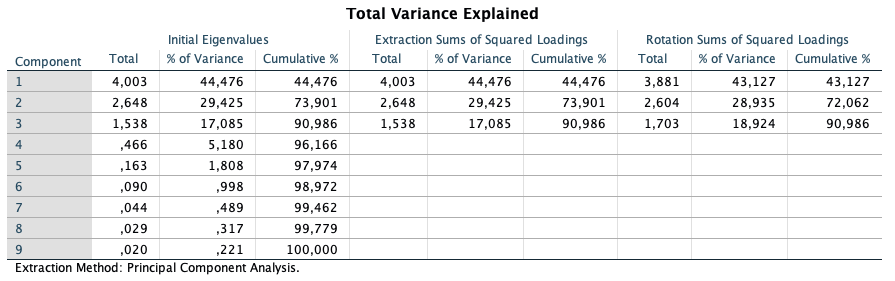
\includegraphics[width=1\textwidth]{Chapters/figures/6_Results/Section2/02_FA_TotalVarianceExplained.png}
\caption{Factor Analysis for OCL metrics}
\label{fig:02_fa_oclmetrics}
\end{figure}

\begin{figure}[ht]
\centering
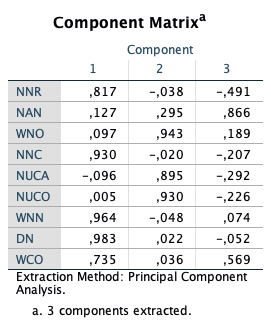
\includegraphics[width=0.35\textwidth]{Chapters/figures/6_Results/Section2/02_FA_ComponentMatrix.png}
\caption{Component Matrix for resulting three components}
\label{fig:02_cm_oclmetrics}
\end{figure}

Using a Binary Logistic Regression, we tried to predict the success of the students considering the three extracted components. Different input methods were tested, but we only achieved very poor results with $R^{2}$ around 3\%.

\begin{comment}

Using a Binary Logistic Regression, we tried to predict the success of the students considering the three extracted components. Different input methods were tested, but we only achieved very poor results with $R^{2}$ around 3\%. Figure~\ref{fig:02_ct_oclmetrics} presents the Classification Table using Forward Stepwise (Likelihood Ratio) method. Prediction for incorrect values showed an acceptable accuracy of 78.8\%, but a weak accuracy of only 24.1\% for the correct values, resulting in a weak prediction percentage of the model of 55.1\%.


\begin{figure}[ht]
\centering
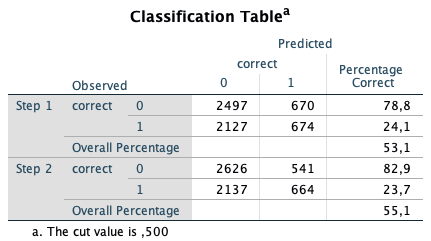
\includegraphics[width=0.5\textwidth]{Template ISCTE-IUL updated/figures/6_Results/Section2/02_FA_ClassificationTable.png}
\caption{Classification table for resulting three components}
\label{fig:02_ct_oclmetrics}
\end{figure}

\end{comment}

The tests described above didn't allow us to conclude that there's a significant correlation between OCL complexity metrics and the success of the students.

\subsection{Readability metrics}

In the previous section, we pursued without success for an explanation of the correctness of students' answers considering the complexity of the solution, i.e., the OCL expression. In this section, we investigate if the explanation can be found instead in the complexity of the problem, i.e., if the complexity of the question posed to the students has a significant influence in the correctness of the responses.

To measure the complexity of the questions, we decided to apply several of the available readability metrics proposed by experts in Literature and Readability over the years~\cite{sanja2013}, which are available in an online tool named Readable~\cite{readable}. For example, for the question \textit{"how many services are provided by TAP?"}, the values for each metric are as seen in Table~\ref{tbl:nlMetricsTap}.

\begin{table}[h]
\centering
\caption{Readability metrics for the given question}
\label{tbl:nlMetricsTap}
\begin{tabular}{@{}ll@{}}
\toprule
Metric                      & Value \\ \midrule
Flesch-Kincaid Grade Level  & 7.4   \\
Gunning Fog Index            & 14.2  \\
Coleman-Liau Index          & 6.0   \\
SMOG Index                 & 11.2  \\
Automated Readability Index & 2.9   \\
FORCAST Grade Level         & 11.4  \\ \bottomrule
\end{tabular}
\quad
\begin{tabular}{@{}ll@{}}
\toprule
Metric                    & Value \\ \midrule
Powers Sumner Kearl Grade & 6.5   \\
Rix Readability           & 6     \\
Flesch Reading Ease       & 54.7  \\
Spache Score              & 3.8   \\
New Dale-Chall Score      & 2.6   \\
Lix Readability           & 36    \\
Lensear Write             & 85.7  \\ \bottomrule
\end{tabular}
\end{table}

Similarly to the OCL complexity metrics, and because we were again facing a high number of variables (total of 13), we decided to assemble a variable reduction. A Kolmogorov-Smirnov test indicates that the majority of the proposed Readability metrics do not follow a normal distribution, D(140) = .089, p = .009 (for Flesch–Kincaid Grade Level, other metrics show similar results). After executing a Spearman’s rho correlation coefficient to evaluate their correlation, and excluding the metrics with strong correlation, we ended up with a smaller set containing the Automated Readability Index, Forest Grade Level, New Dale-Chall, and Lensear Write. Applying a Linear Regression to assess the capability of the resulting metrics to explain the correctness of the answers, a significant regression equation was found F(4, 135) = 6.311, $p<.001$, with an $R^{2}$ of .158. The resulting linear model revealed once again a poor explanatory power on the success of the students.


\begin{comment}
\begin{figure}[ht]
\centering
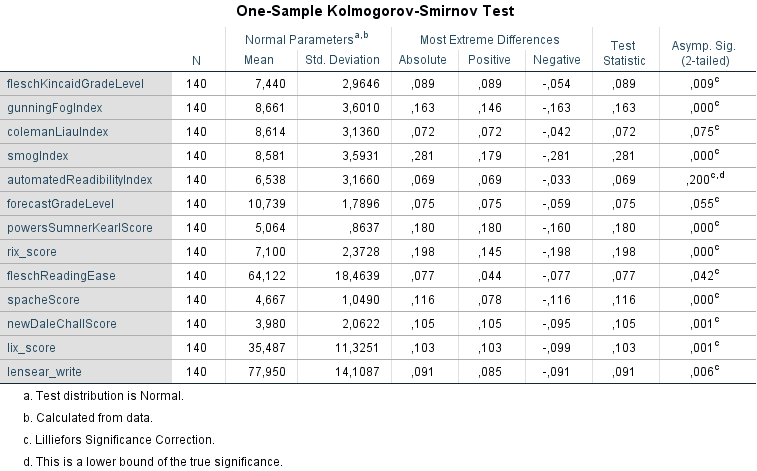
\includegraphics[width=1\textwidth]{Template/Chapters/figures/6_Results/Section2/02_KS_NLmetrics}
\caption{Kolmogorov–Smirnov test on the normal distribution of Readability metrics}
\label{fig:02_ks_nlmetrics}
\end{figure}

\begin{figure}[!h]
\centering
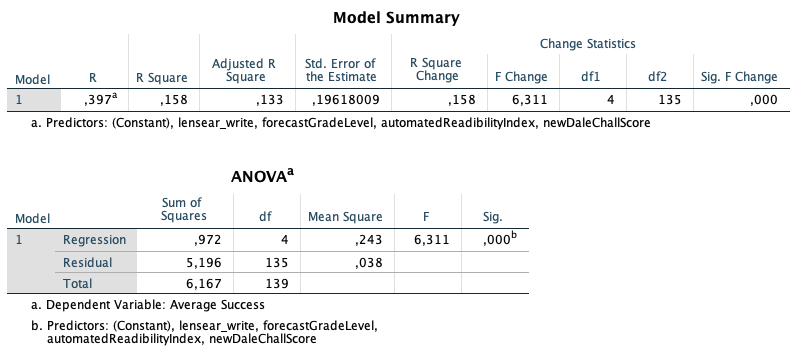
\includegraphics[width=0.48\textwidth]{Figures/SPSS/02_LR_NLmetrics.png}
\caption{Linear Regression using Automated Readability Index, Forest Grade Level, New Dale-Chall, and Lensear Write to explain the success}
\label{fig:02_lr_nlmetrics}
\end{figure}
\end{comment}

In conclusion, our tests show that neither the complexity of the questions, given by Readability metrics, nor the complexity of the answers, given by OCL complexity metrics, can be used to explain the success of the students when answering the questionnaires.

\section{Experiment 3: On the Effect of Using the OCL Highlight Plugin}
\label{chap:Results-OCLHighlightPlugin}

In this last section of experiments, we focus on understanding whether the OCL Highlight Plugin was able to soften the learning curve when studying OCL and therefore produced the desired effect for which it was intended. Before requesting the students to use the plugin on their final questionnaires, it was important to have a stable version. The development of the plugin required several iterations, which allowed for the correction of bugs and also the introduction of “nice-to-have” features, such as the configuration of the highlight colours. The feedback on the stability and usefulness of the plugin was first questioned to experts in the field. After making the necessary corrections, the students were able to experiment with the plugin during the semester. On the day of the exam, we collected their answers, and by comparing the results to the ones obtained in previous school years, we were able to discern the positive impact of the plugin.

\subsection{Qualitative evaluation: experts}
\label{chap:Results-pluginExperts}

In this subsection, we present the focus group study we conducted to obtain feedback and experiences
from UML/OCL experts (teachers) when using the OCL Highlight Plugin to teach OCL to undergraduate students at the university. This experience followed the available guidelines on how to plan and run focus groups~\cite{Kontio2004}:

\paragraph{Defining the research problem:} The objective of the study was to provide insights into the utility of the developed plugin to ease the learning of OCL from the perspective of UML/OCL experts (teachers). Furthermore, we sought to obtain suggestions for improvement and the teachers' opinions on how students reacted to it.

\paragraph{Selecting the participants:} Six teachers from the Department of Computer Science at ISCTE were invited by e-mail to take part in the focus group discussions. The selected invitees are Software Engineering experts, and they teach UML and OCL to bachelor students.

\paragraph{Planning and conducting the focus group session:} We designed the focus group session to consist of two parts. On the first part, teachers were asked to individually observe their respective students during a week of classes, where students were submitted to their first contact with USE and the plugin. At the end of the week, teachers were invited to attend a one-hour meeting to discuss their observations and fill out a previously prepared short questionnaire about the usefulness of the plugin and the reaction of students to it.

\paragraph{Analysis:} Results in Table~\ref{tbl:pluginValidation} indicate that UML/OCL experts agreed on the usefulness of the plugin and that it helps students to understand how OCL transverses a class diagram. This assessment showed that students could easily operate with the plugin, as we did not want to aggravate the difficulty in learning by introducing another element that they would need to manage. As a last remark, some teachers also referred that students thought that the highlighting was something obvious, which again might indicate that it provides a natural integration with the tool.

% Please add the following required packages to your document preamble:
% \usepackage[normalem]{ulem}
% \useunder{\uline}{\ul}{}

%\begin{tabular}{p{0.25\linewidth}p{0.25\linewidth}p{0.25\linewidth}}
\begin{table*}[ht]
\scriptsize
    \centering
    
    \caption{Qualitative Validation of the OCL Highlight Plugin}
    
    \label{tbl:pluginValidation}
    
    \begin{tabular}{cll}
        
        \hline
        
        \\
        
        \multicolumn{1}{l}{}QUESTIONS & 
        %\begin{tabular}[c]{@{}l@{}}
        \begin{tabular}[c]{m{5.5cm}}
            What is your opinion, as a UML/OCL expert, on the usefulness of this plugin? Considering that you have used the tool without the plugin, do you think it can  help students when learning OCL? \\ \\
        \end{tabular}
        
        \begin{tabular}[c]{m{5.5cm}} 
            How did the students in your class(es) react to the plugin? In particular, the assimilation of the visual metaphor was easy, that is the correspondence between the textual expression in OCL and the highlighted elements in the class diagram? \\ \\
        \end{tabular}
        
        \\
        
        \hline
        
        \\
        
        \begin{tabular}[c]{m{1cm}}
            Expert 1
        \end{tabular} &
        
        \begin{tabular}[c]{p{5.5cm}}
            An indispensable and missing plugin, so far! While learning OCL, it is critical to understand the relationship between the often complex OCL expressions and related modeling elements defined in a class diagram – often complex as well. OCL Highlight plugin delivers a simple, yet complete, graphical representation of those relationships, thus facilitating the understanding and learning of OCL expressions.
        \end{tabular}
        
        \begin{tabular}[c]{p{5.5cm}}
            The students quickly understood the usefulness and ease of use of the plugin. The visual matching between the OCL expression and the related modeling elements in the class diagram was considered very intuitive. The graphical feedback also motivated the students to try out and understand increasingly complex OCL expressions.
        \end{tabular} 
        
        \\
        
        \begin{tabular}[c]{m{1cm}}
            Expert 2
        \end{tabular} & 
        
        %\begin{tabular}[c]{@{}l@{}}
        \begin{tabular}[c]{m{5.5cm}}
            I consider that the plugin is of great utility since it illustrates the navigation of the queries in OCL. It facilitates the understanding of the expressions, as well as the understanding of OCL language.
        \end{tabular}
        
        \begin{tabular}[c]{m{5.5cm}}
            The reaction of the students to the plugin was something natural as if it was something obvious that the tool "painted the way". I took the opportunity of asking them if the path was not painted in the class diagram would be more difficult to understand the semantics of queries, and most students said yes.
        \end{tabular}
        
        \\
        
        \begin{tabular}[c]{m{1cm}}
            Expert 3
        \end{tabular} &
        
        \begin{tabular}[c]{m{5.5cm}}
            The plugin is extremely important as students have some difficulties to understand OCL and, more importantly, to build OCL expressions. This visual insight helps to grasp how OCL operates over the model.
        \end{tabular}
        
        \begin{tabular}[c]{m{5.5cm}}
            Yes, they have immediately realized which parts of the model were involved.
        \end{tabular}                                                               
        
        \\
        
                \begin{tabular}[c]{m{1cm}}
            Expert 4
        \end{tabular} &
        
        \begin{tabular}[c]{m{5.5cm}}
            It is a very useful plugin since it helps the students understand what classes are being used in each OCL expression. It introduces traceability and shows a better insight to the students, making it easier for them to learn.
        \end{tabular}
        
        \begin{tabular}[c]{m{5.5cm}}
            Yes, they understood quickly how OCL expressions worked.
        \end{tabular}
        
        \\
    
        \begin{tabular}[c]{m{1cm}}
            Expert 5
        \end{tabular} &
        
        \begin{tabular}[c]{m{5.5cm}}
            This plugin is mostly a good facilitator and a really useful tool for the understanding of UML/OCL, mainly when we have class diagrams with a considerable size. Especially for students, it can ease and improve the process of learning OCL queries.
        \end{tabular}
        
        \begin{tabular}[c]{m{5.5cm}}
            In class and with this plugin, students were able to follow the OCL expressions they were writing by immediately visualizing the result of those queries in terms of the used classes, associations and attributes that were highlighted. Students accepted the use of this tool really well, compared with the previous year, it not only provided a more engaging learning experience for the students but also, as a lecturer, it helped to demonstrate the process of querying.
        \end{tabular} 
        
        \\
        
        \begin{tabular}[c]{m{1cm}}
            Expert 6
        \end{tabular} &
        
        \begin{tabular}[c]{m{5.5cm}}
            I believe that, in fact, this plugin can facilitate the learning of OCL by the students. The selective visualization allows a greater concentration and effectiveness of the analysis of the pathway performed by the queries.
        \end{tabular}
        
        \begin{tabular}[c]{m{5.5cm}}
            The students in my class seemed to assimilate well the connection between the path highlighted in the diagram and the path made by the OCL queries.
        \end{tabular}
        
           \\ \\
        
        \hline
    
    \end{tabular}

\end{table*}


\subsubsection{Quantitative evaluation: students}
\label{chap:Results-pluginStudents}

As a last set of experiments, we explore the impact of the usage of the plugin on students' answers. To consider it a success, we aspire to observe a significant increase in correct answers, when comparing to previous school years where the courses were given without the plugin. We are also interested in observing how the duration of the questionnaires was affected.
For this analysis, we only considered the school years 2 and 5 because they used the same model, in an attempt to isolate the effect of using different models. Since the e-learning platform didn't allow to collect the time the students took per question in year 2 (only the cumulative time of the test was available), we grouped the total of correct answers per test. 
On the matter of test duration, a Levene's test found that the assumption of homogeneity of variance between the groups (test duration and usage of the plugin) was violated, $p<.01$; therefore we carried out a two-tailed independent samples T-Test based on unequal variances. The test duration with plugin (M=2012.91, SD=398.554) is accepted as similar when compared to not using the plugin (M=1942.59, SD=257.579), t(-1.968)=332.825, $p=.05$ (Figure~\ref{fig:03_TTest_Duration}). With a p-value at the limit of rejection, we assume from the calculated average values that the time consumption is very similar, despite being slightly superior when using the plugin.

\begin{figure}[ht]
\centering
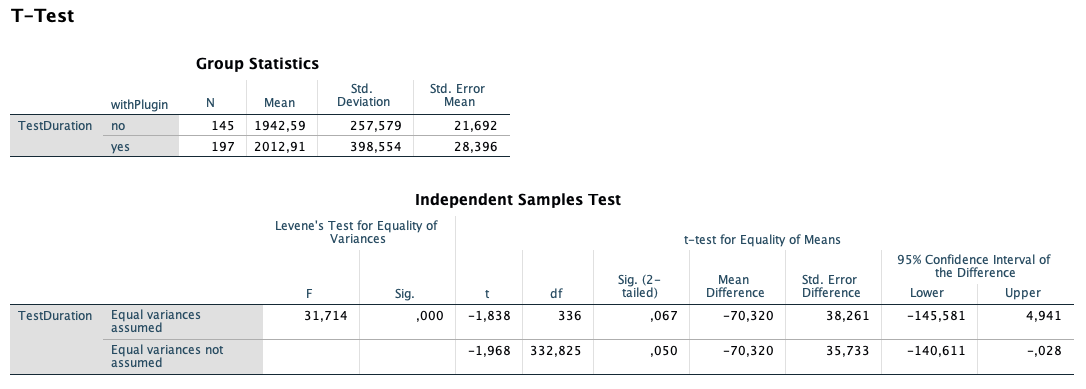
\includegraphics[width=1\textwidth]{Template/Chapters/figures/6_Results/Section3/03_TTest_Duration.png}
\caption{Independent Samples T-Test between test duration and usage of the plugin}
\label{fig:03_TTest_Duration}
\end{figure}

A similar analysis was made, this time considering the correct answers. The equality of variances was met using a Levene’s test, $p>.05$. An independent samples T-Test for equal variances showed that the number of correct answers was significantly higher when using the plugin (M=5.45, SD=2.807) than when not using it (M=3.63, SD=2.879), t(-5.836)=340, $p<.05$ (Figure~\ref{fig:03_TTest_Correct}).


\begin{figure}[ht]
\centering
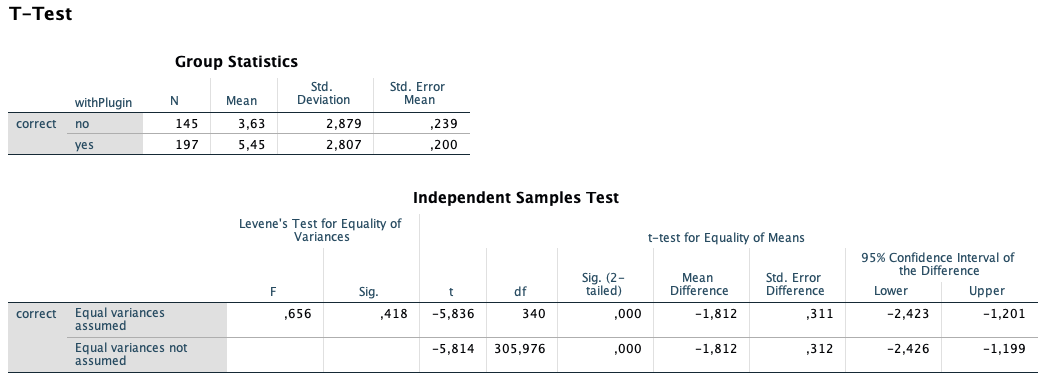
\includegraphics[width=1\textwidth]{Template/Chapters/figures/6_Results/Section3/03_TTest_Correct.png}
\caption{Independent Samples T-Test between total of correct answers and usage of the plugin}
\label{fig:03_TTest_Correct}
\end{figure}

The analyses presented above allow us to conclude that even though there was a slight increase in the amount of time used by the students to complete the questionnaires, it was not significant. On the other hand, the grades (amount of correct answers) revealed a notable improvement. With these tests, we inferred that using the plugin proved to be beneficial to students when learning OCL, and did not introduce an additional effort that would reduce the speed of response of the questionnaires.

A Chi-Square test of independence confirmed this conclusion, showing that there is a significant association between using the plugin and the correctness of the answers, $\chi^{2}$(1, N = 3420) = 110.177, $p<.01$ (Figure~\ref{fig:03_Plugin_Chi_Square_Subset}). We obtained a similar result when performing the same test against the whole dataset (years 1 to 5), $\chi^{2}$(1, N = 6300) = 80.538, $p<.01$.

\begin{figure}[ht]
\centering
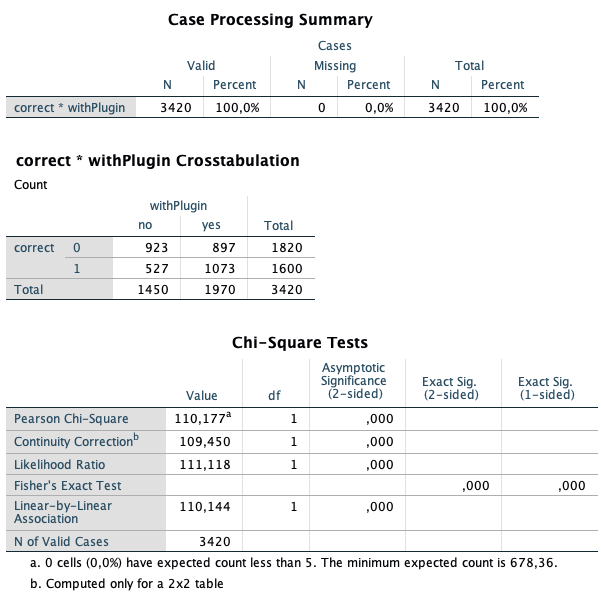
\includegraphics[width=0.7\textwidth]{Template/Chapters/figures/6_Results/Section3/03_Plugin_Chi_Square_Subset.png}
\caption{Chi-Square test for the association between answer's correctness and usage of the plugin}
\label{fig:03_Plugin_Chi_Square_Subset}
\end{figure}

As a last test, it is crucial to prove that there was no difference between the complexity of the questions and answers on both years, as that would jeopardize our experiences. Assuming equal variances between the complexity of the questions in years 2 and 5 (Levene's test with $p>.01$), a T-Test shows that there was no significant difference between the groups, $p>.01$ (see Figure~\ref{fig:03_TTest_NLMetrics}). The same test applied to OCL complexity metrics requires a deeper analysis, as the results for each metric are dissimilar (see Figure~\ref{fig:03_TTest_OCLMetrics}): assuming equal variances for NNR, NNC and DN (Levene's test, $p>.01$), there is no significant difference between both groups, $p>.01$; assuming equal variances for NAN (Levene's test, $p>.01$), complexity of answers in year 2 is significantly higher when compared to year 5, $p<.01, t>0$; assuming unequal variances for WNO, NUCA and WNN (Levene's test, $p<.01$), there is no significant difference between groups, $p>.01$; assuming unequal variances for WCO (Levene's test, $p<.01$), complexity of answers in year 2 is again significantly higher than in year 5, $p<.01, t>0$. 

\begin{figure}[ht]
\centering
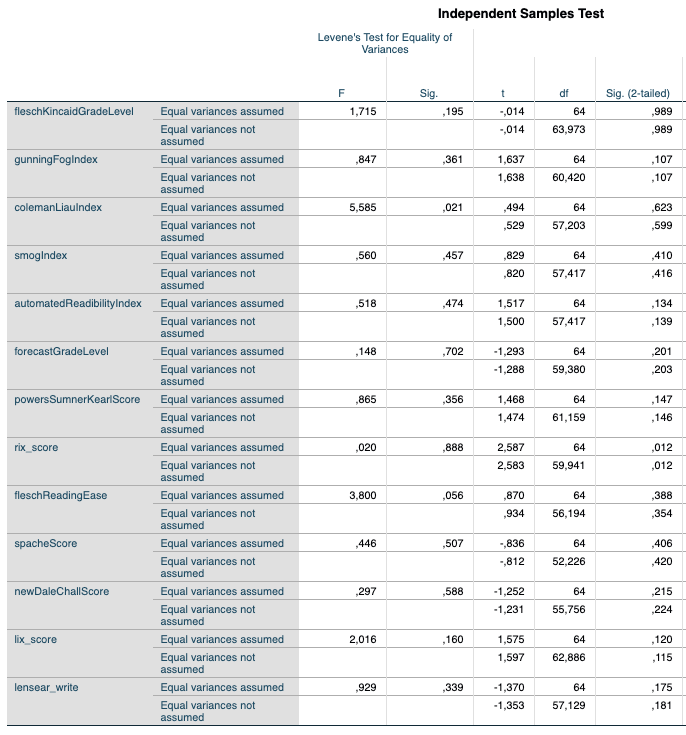
\includegraphics[width=1\textwidth]{Template/Chapters/figures/6_Results/Section3/03_TTest_NLMetrics.png}
\caption{Independent Samples T-Test between the readability metrics of years 2 and 5}
\label{fig:03_TTest_NLMetrics}
\end{figure}

\begin{figure}[ht]
\centering
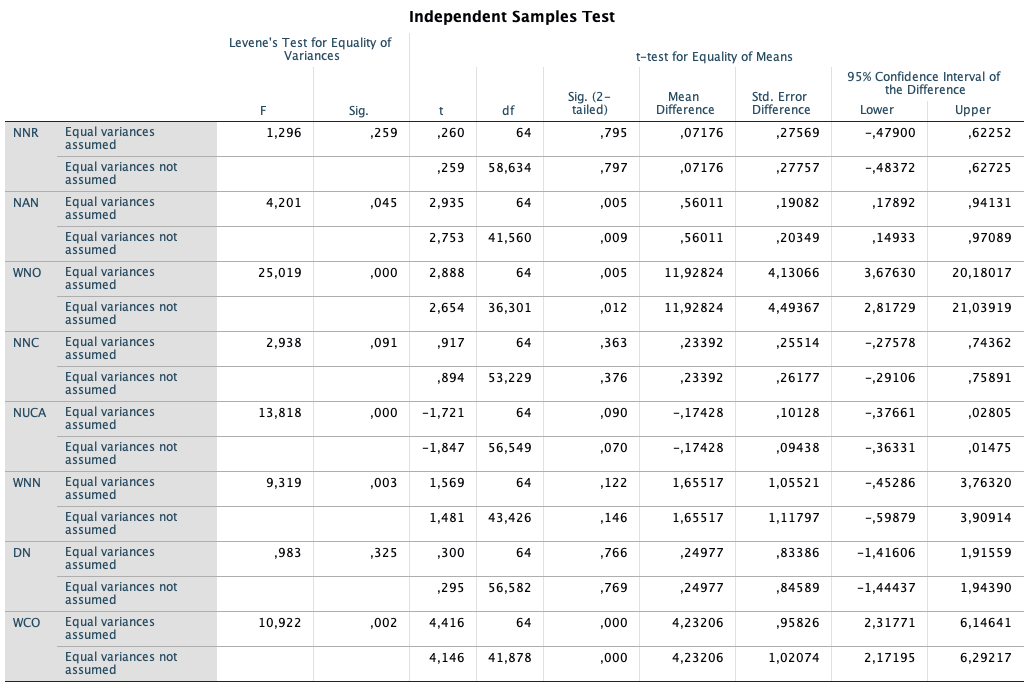
\includegraphics[width=1\textwidth]{Template/Chapters/figures/6_Results/Section3/03_TTest_OCLMetrics.png}
\caption{Independent Samples T-Test between the OCL complexity metrics of years 2 and 5}
\label{fig:03_TTest_OCLMetrics}
\end{figure}

\begin{comment}
An initial chi-square test of independence showed that there is a significant association between using the plugin and the correctness of the answer, $\chi^{2}$(1, N = 6300) = 80.538, $p<.01$ (see Figure~\ref{fig:03_Plugin_Chi_Square}).

\begin{figure}[ht]
\centering
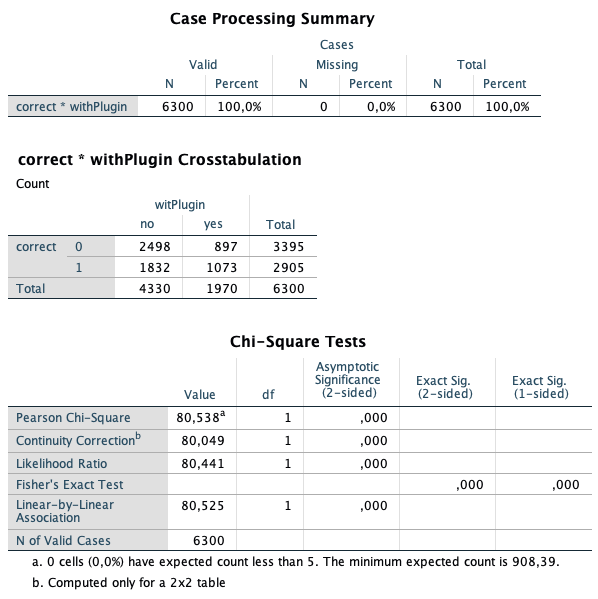
\includegraphics[width=0.7\textwidth]{Chapters/figures/6_Results/Section3/03_Plugin_Chi_Square.png}
\caption{Chi-Square test for the association between answer's correctness and usage of the plugin}
\label{fig:03_Plugin_Chi_Square}
\end{figure}


Our result is statistically significant, i.e, we accept the alternative hypothesis which states that there is a significance association between answer's correctness and usage of the plugin. Correctness is not independent of the usage of the plugin.
$\chi^{2}$(1, N = 6300) = 80.538, $p<.01$
\end{comment}








